%Version 3.1 December 2024

\documentclass[pdflatex,twocolumn,sn-mathphys-num]{sn-jnl}

\usepackage{algorithm}
\usepackage{algorithmicx}
\usepackage{algpseudocode}
\usepackage{amsmath,amssymb,amsfonts}
\usepackage{amsthm}
\usepackage[title]{appendix}
\usepackage{booktabs}
\usepackage{bm}
%% \usepackage{dblfloatfix}
\usepackage{graphicx}
%% \usepackage[margin=0.75in, paperwidth=8.5in, paperheight=11in]{geometry}
\usepackage[margin=0.75in, left=2.75in, right=2.75in, paperwidth=12.5in, paperheight=11in]{geometry}
\usepackage{harpoon}
\usepackage[utf8x]{inputenc}
\usepackage{layout}
\usepackage{listings}
\usepackage{manyfoot}
\usepackage{makecell}
\usepackage{mathrsfs}
\usepackage{multirow}
\usepackage{subcaption}
\usepackage{svg}
\usepackage{textcomp}
\usepackage{xcolor}


%% ================= MACROS ======================

\newcommand{\vc}[1]{\overrightharp{#1}}
\newcommand{\bb}[1]{\mathbb{#1}}
\newcommand{\dif}{\mathop{}\!\mathrm{d}}



\raggedbottom
%%\unnumbered% uncomment this for unnumbered level heads

%% ================== TITLE PAGE ==================

\begin{document}

\title[Tomographic Retrieval of the Optically Thin Exosphere]{Tomographic Retrieval of the Optically Thin Exosphere}

\author{\fnm{Evan} \sur{Widloski}}\email{evanw3@illinois.edu}
\author{\fnm{Lara} \sur{Waldrop}}\email{lwaldrop@illinois.edu}

\affil{\orgdiv{Electrical and Computer Engineering}, \orgname{University of Illinois Urbana-Champaign}, \orgaddress{\street{306 N Wright}, \city{Champaign}, \postcode{61820}, \state{IL}, \country{United States}}}


\abstract{The abstract serves both as a general introduction to the topic and as a brief, non-technical summary of the main results and their implications. Authors are advised to check the author instructions for the journal they are submitting to for word limits and if structural elements like subheadings, citations, or equations are permitted.}

\keywords{remote sensing, tomography, spacecraft, inverse problems, exosphere, geocorona}

%%\pacs[JEL Classification]{D8, H51}

%%\pacs[MSC Classification]{35A01, 65L10, 65L12, 65L20, 65L70}

\maketitle

%% ================== BODY ==================

\section{Introduction}\label{intro}

TO BE FILLED BY LARA


\section{Measurements and Emission Model}
\label{sec:measurement_constraints}

This section will describe the Carruthers orbit, camera geometry, an emission model of Lyman-$\alpha$ interaction with and propagation through exospheric hydrogen, instrument model overview, and end with the post-processing procedure for converting raw sensor measurements to salient science constraints.

  The Geocentric Solar Ecliptic (GSE) coordinate system is a natural fit when describing spacecraft position and the exospheric hydrogen distribution, since radiation pressure is expected to impose Sun-Earth alignment on global exospheric structure.  The rest of this manuscript uses GSE in units of Earth radii (1 Re = 6371 km) either in cartesian or spherical coordinates.

  Carruthers will be inserted into a halo orbit around the L1 Lagrange point (about 1.5 million km from Earth, 235 Re), which is distant enough to observe the entirety of the geocorona from an outside vantage
  over its mission lifetime \cite{baliukin}.

  This orbit deviates above/below the ecliptic plane by ±7° (31 Re) and ±28° (112 Re) in the dawn/dusk direction from the Sun-Earth line, providing angular measurement diversity for tomographic analysis of the exosphere, shown in Figure \ref{fig:orbit_details}.

Carruthers is equipped with two co-aligned UV cameras and will observe global exospheric emission at Lyman-$\alpha$ from a distant vantage, providing constraints on the global distribution of hydrogen.
The Narrow Field Imager (NFI) observes the inner exosphere at high resolution on a 30 minute cadence and the Wide Field Imager (WFI) observes global distribution of exospheric hydrogen on a 60 minute cadence.
  A summary of camera geometry specifications is given in Table \ref{tab:camera_specs}.

  \begin{table*}[h]
    \centering
    %% \setlength{\tabcolsep}{4pt} % Default value: 6pt
    \caption{Camera geometry specifications. Spatial resolution is projected onto Earth tangent plane as in Figure \ref{fig:fov}.  Vantage-dependent specifications computed at orbit perigee/apogee of 190/265 Re}%
    \begin{tabular}{@{}cccccc@{}}
      \toprule
      %% Camera & FOV (degrees) & Resolution (pixels) & Angular Res. (degrees) & Spatial Res. (Re, proj.) & FOV Radius (min-max Re) \\
      \thead{Camera} &
      \thead{FOV \\ (degrees)} &
      \thead{Resolution \\ (pixels)} &
      \thead{Angular Res. \\ (degrees)} &
      \thead{Spatial Res. \\ (Re, proj.)} &
      \thead{FOV Radius \\ (min-max Re)} \\
      \midrule
          WFI & 18° & 512² & $35*10^{-3}$ & 0.12 - 0.16 & 6.0 - 8.3 \\
          NFI & 3.6° & 1024² & $3.5*10^{-3}$ & 0.059 - 0.081 & 30 - 42 \\
      \botrule
    \end{tabular}
    \label{tab:camera_specs}
  \end{table*}

  Together, these cameras are capable of measuring both the fast-evolving dynamics of the inner exosphere and the global distribution of hydrogen along with the interplanetary background Lyman-$\alpha$ signal (discussed in the next section).  Figure \ref{fig:fov} shows the field of view (FOV) of the cameras relative to the inner exosphere boundary and outer exospheric limit.


\begin{figure}[h]
  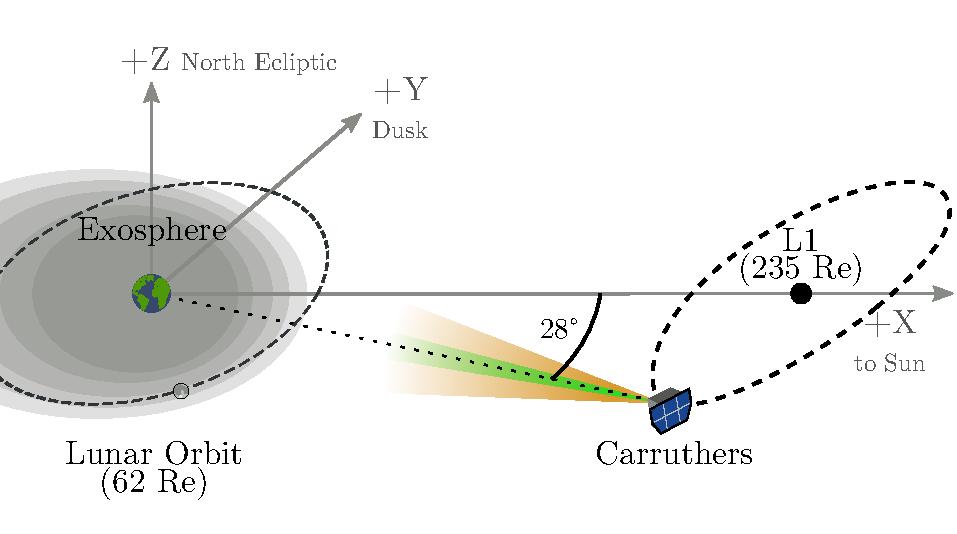
\includegraphics[width=1\linewidth]{figures/orbit}
  \caption{6 month Carruthers orbit around L1.  Not to scale.}
  %% \footnotetext{Earth/Moon image courtesy of https://de.wikipedia.org/wiki/Benutzer:Master_Uegly}
  \label{fig:orbit_details}
\end{figure}

\begin{figure}[h]
  \center
  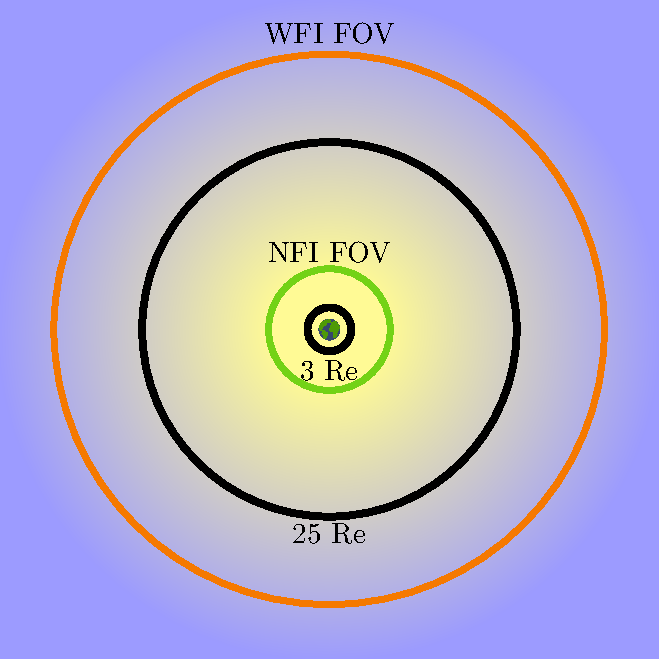
\includegraphics[width=.6\linewidth]{figures/fov}
  \caption{Carruthers camera FOV projected onto Earth tangent plane. FOV relative to retrieval boundaries.}
  \label{fig:fov}
\end{figure}


%% =============== EMISSION MODEL =================


In order to recover a hydrogen density distribution from measurements, it is necessary to mathematically model how Lyman-$\alpha$ photons propagate through the exosphere and enter the camera.
This is known as an emission model and is a central component of tomographic retrieval algorithms.

  Numerically modeling the physics of radiative transfer is a computationally complex task, as solar Lyman-$\alpha$ photons entering the atmosphere usually scatter multiple times, creating nonlinear interdependencies between distant portions of the exosphere.  However, in regions of the atmosphere where hydrogen is sparse (known as the optically thin regime) it is a valid approximation that incident solar photons resonantly scatter only once \cite{ostgaard}, simplifying computational requirements and implementation complexity of the emission model.

  Anderson and Hord Jr. \cite{opticaldepththin} define the optically thin regime as starting when $\tau <= 0.1$, where optical depth $\tau$ is a measure of the proportion of photons scattering only once.

  With these assumptions, the measurement by the spacecraft is proportional to a line integral of the total mass of hydrogen present in the atmosphere along the LOS of a particular pixel, given by photon radiance

  \begin{equation*}
    I_{\text{exo},t} = \frac{g_t}{4 \pi} \phi (\beta)
    \int_S \bm{a}_t (\vc{s}) \bm{\rho}_t (\vc{s}) \dif s
    \text{  (phot/s/cm²/sr) }
  \end{equation*}

    %% #gt([(phot/s/cm²/sr)])

  where $S$ is the pixel LOS, $g_t$ is solar g factor, $t$ is time, $\phi$ is the scattering phase function, $\bm{a}_t$ is albedo correction factor, $\vc{s}$ is position vector and $\bm{\rho}$ is hydrogen density, illustrated in Figure \ref{fig:emission_model_physics}.
  Table \ref{tab:emission_units} gives an overview of different measurement quantities and their units.

  $I_{\text{exo}_t}$ is line-integrated radiance, an integral over wavelength of the Lyman-$\alpha$ emission line whose width is due to thermal broadening.

\begin{figure}[h]
  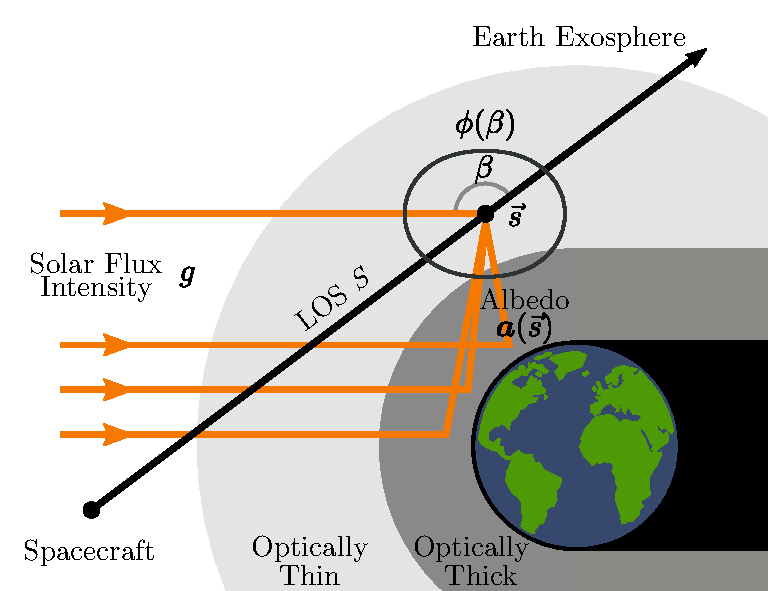
\includegraphics[width=.9\linewidth]{figures/physics}
  \caption{Emission model overview for a LOS. Not to scale.}
  \label{fig:emission_model_physics}
\end{figure}

\begin{table}[h]
  \centering
  %% \setlength{\tabcolsep}{4pt} % Default value: 6pt
  \caption{Quantities involved in emission model and their units.}
  \begin{tabular}{@{}lcc@{}}
    \toprule
    \thead{Quantity} & \thead{Symbol} & \thead{Units} \\
    \midrule
    Density & $\bm{\rho}$ & atom/cm³ \\
    Line-integrated radiance & $I_{\text{exo}}$ & phot/s/atom/cm²/sr \\
    Angular g factor & $g$ & phot/s/atom/sr \\
    Albedo correction factor & $\bm{a}$ & unitless \\
    Scattering phase function & $\phi$ & unitless \\
    \botrule
  \end{tabular}
  \label{tab:emission_units}
\end{table}

The scattering phase function $\phi$ represents the directional distribution of resonantly-scattered photons relative to the direction of the Sun @chamberlain.

The solar g factor $g_t$ (phot/s/atom) relates hydrogen density (atoms/cm³) to photon flux emitted per unit volume (phot/s/cm³) \cite{gfactor}.   The quantity $g_t / (4 \pi) \phi(\beta)$ describes the rate of photons being emitted into a part of the sky (1 steradian) from a unit volume of gas and is assumed to be a known, external input to the emission model.  The solar g factor is proportional to incident solar Lyman-α flux at line center, which is time-varying and measured on-orbit.

    Finally, $\bm{a}_t (\vc{s})$ is a unitless multiplicative correction factor (assumed known) to account for high-density regions of the inner optically thick exosphere which act as a secondary source of Lyman-α photons illuminating the outer exosphere from below.

Zoennchen et al. \cite{zoennchen_new} have found that extending the optically thin model to include extinction along the LOS and extinction between the Sun and scattering point reduced discrepancy between tomographic retrievals and physics-based simulations.  The scope of this manuscript does not include these correction terms but may be included in a future work.

A tenuous distribution of hydrogen throughout the solar system, known as IPH, also contributes to the line-integrated Lyman-α radiance detected by the spacecraft.
  IPH, like solar g factor, will be measured independently by Carruthers and is assumed to be known.
  The impact of biases introduced by IPH subtraction has been considered to make sure retrievals still meet error requirements.
    Other unwanted sources of Lyman-α signal which violate emission model assumptions include the Moon and stars and the optically thick exosphere, as shown in @masks, but these sources will be masked and not used as retrieval constraints.  Together, these radiance sources are referred to as $I_\text{bkg}$.


%% ======================== PREPROCESSING ======================

\section{Preprocessing}

Raw sensor measurements (digital number, DN) must be calibrated to column densities (atoms/cm²) before they can be ingested by the retrieval algorithm.
  The details of calibration are out of scope of this manuscript, but can be found in (FIXME: cite Alex calibration paper.)

  Calibration reverses many of the terms of the emission model given in the previous section and additional distortion introduced by the instrument, resulting in an expression for column density that is independent of any instrument parameters or solar conditions

    \begin{equation}
        y_{t j} \approx \int_{S_{t j}} \bm{a}_t (\vc{s}) \bm{\rho}_t (\vc{s}) \dif s \text{  (atom/cm²)}
    \end{equation}

  where LOS $S_{t j}$ is annotated with indices $t j$ to emphasize time and pixel dependence.

    As mentioned previously, some LOS contain Lyman-$\alpha$ signals which are unknown or violate the emission model assumptions and must be marked so they are ignored during retrieval.  These include the Moon, stars, optically thick exosphere, and Earth shadow, shown in Figure \ref{fig:masks} \cite{zoennchen_old}.

\begin{figure*}[t!]
  \centering
  \begin{subfigure}[t]{0.3\textwidth}
    \centering
    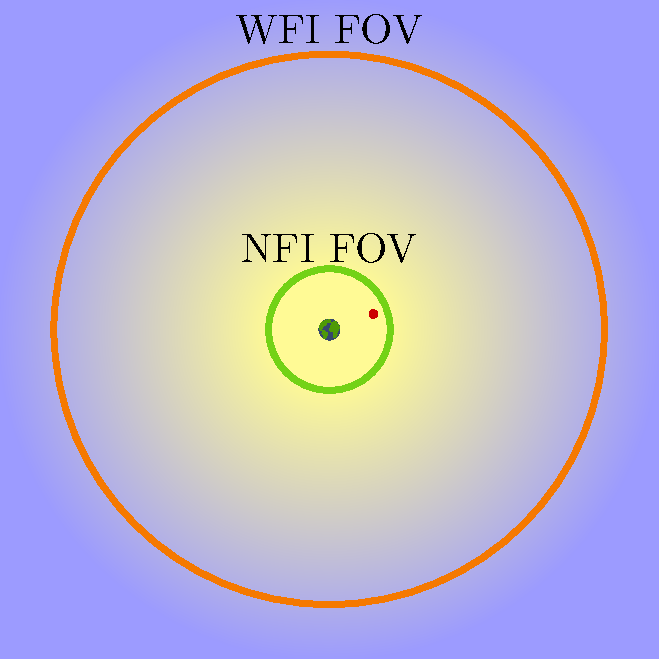
\includegraphics[height=1.8in]{figures/mask_moon}
    \caption{Moon mask}
  \end{subfigure}%
  \begin{subfigure}[t]{0.3\textwidth}
    \centering
    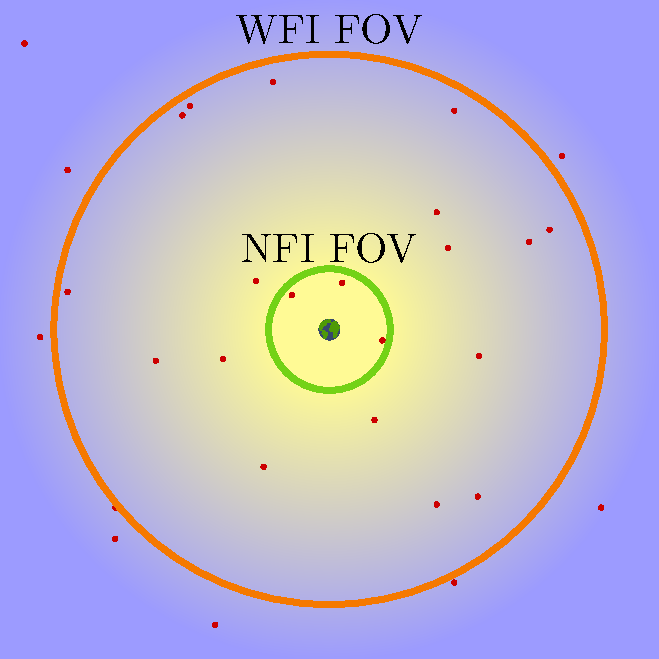
\includegraphics[height=1.8in]{figures/mask_stars}
    \caption{Stellar mask}
  \end{subfigure}
  \begin{subfigure}[t]{0.3\textwidth}
    \centering
    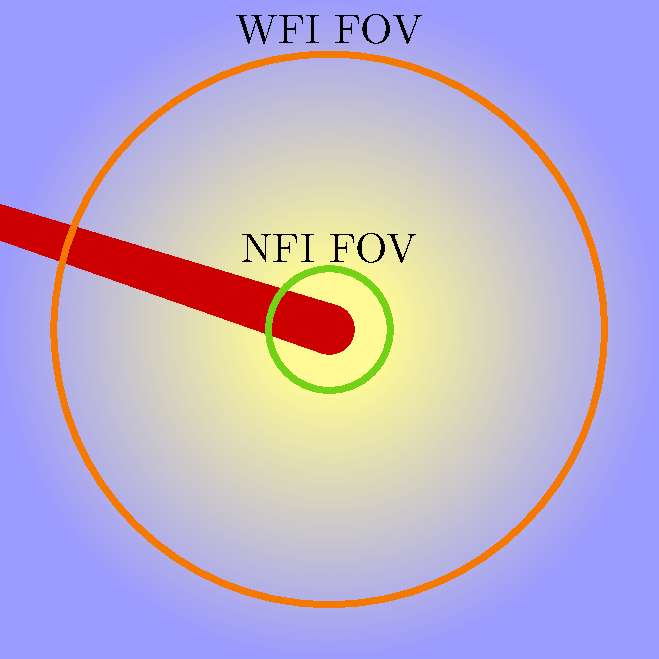
\includegraphics[height=1.8in]{figures/mask_thick}
    \caption{Optically thick exosphere and shadow mask}
  \end{subfigure}
  \caption{Extraneous sources of Lyman-$\alpha$ that must be masked, relative to NFI/WFI camera FOV}
  \label{fig:masks}
\end{figure*}

\begin{figure}[h]
  \centering
  \begin{subfigure}[t]{0.50\linewidth}
    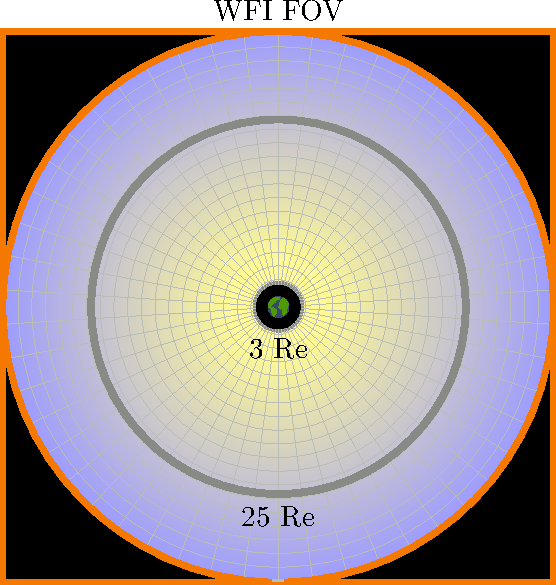
\includegraphics[height=1.7in]{figures/polar_fov_wfi}
    \caption{WFI}
  \end{subfigure}%
  \begin{subfigure}[t]{0.50\linewidth}
    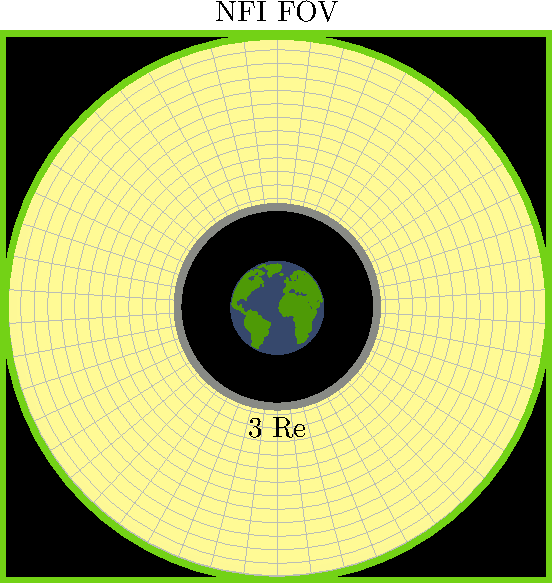
\includegraphics[height=1.7in]{figures/polar_fov_nfi}
    \caption{NFI}
  \end{subfigure}
  \caption{Polar-binning for WFI and NFI cameras reduces computational burden with minimal information loss.  Actual radial bin size is down-sampled by 5x for visualization.}
  \label{fig:earth_fov_science}
\end{figure}

  A final step of post-processing is to bin the native 512² pixel WFI and 1024² pixel NFI images to a lower resolution.  The dense LOS spatial sampling and fast temporal cadence of these cameras creates significant memory and computational requirements for the retrieval algorithm, which can be avoided by downsampling images in a way that preserves as much detail as possible.  This downsampling is similar to the stacking and binning described in (FIXME: cite Alex paper), but occurs after downlink.  A polar binning scheme is well-suited for retrievals due to the roughly spherically-symmetric distribution of the exosphere.  Within the Carruthers mission, this is referred to as science pixel binning and shown in Figure \ref{fig:earth_fov_science}. Similarly, temporal averaging can reduce the volume of data ingested by the retrieval algorithms without much loss of information on exosphere dynamic evolution, especially during geomagnetically quiet conditions.  The corners of the detector are clipped as they are blocked by the instrument's circular apertures and contain no Lyman-$\alpha$ data.  These data reduction techniques improve the memory resources required during retrieval and without significant loss of information for the particular spatial and temporal binning parameters chosen.

    This section has focused on treating a single detector pixel $j$ and associated LOS at a single time index $t$ for the sake of notational simplicity, but tomographic retrieval algorithms rely on many measurements from different angles to fully constrain a reconstruction.
    This manuscript uses the convention $\bm{y} = \{y_{t,j} | \forall t, \forall j\}$ to denote a stack of calibrated 2D measurements, which will be used to retrieve a 3D H density distribution in the next chapter.


%% ======================== INVERSE PROBLEM ======================


\section{Inverse Problem Formulation and Density Model}\label{sec:inverse_problem}

An inverse problem is the procedure of determining the causative factors of a set of measurements derived from an observation process.  In exospheric tomography, the factor driving the magnitude of column density measurements is the density distribution of hydrogen in the regions being observed.  Figure \ref{fig:inverse_problem_schematic} shows a generalized example of an inverse problem

\begin{figure}[h]
  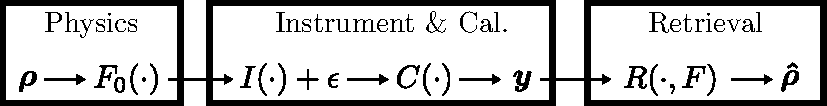
\includegraphics[width=1\linewidth]{figures/inverse_problem}
  \caption{General schematic for an observing system and inverse problem}
  \label{fig:inverse_problem_schematic}
\end{figure}

where $\bm{\rho}$ and $\bm{\hat{\rho}}$ are the ground truth and estimated density distribution, $I$ and $C$ are instrument model and calibration, $\bm{y}$ are column density measurements, $\epsilon$ is measurement noise,  $R$ is a retrieval algorithm, and $F_0$ is a forward tomographic operator describing reality while $F$ is a numerical approximation.  This distinction between forward operators matters when considering model uncertainty or mismatch discussed in (FIXME: remove this reference, will not include in paper).

\subsection{Discretization}\label{sec:discretization}

In general, direct analytic solutions to tomographic estimation problems are infeasible, necessitating a numerical approach where the solution space is divided into a finite grid of $N$ non-overlapping regions called voxels where density is assumed to be constant.  There are a large variety of grid types to choose from, including regular grids (e.g. spherical, cylindrical, cartesian), non-regular grids which may utilize hierarchical structures (e.g. octree) and tetrahedral meshes.
Some of these discretizations schemes have been designed to adaptively update voxel boundaries during retrieval to better fit the object being retrieved \cite{adaptivemesh1}.

Choosing a discretization grid which is well-suited to the data is critical, as an improper grid can create aliasing and other artifacts that cause the numerical result to deviate from the functions they approximate.  Since the exosphere is well-understood to smoothly vary with larger density gradients at lower altitudes, a regular spherical grid with logarithmically spaced radial bins is appropriate.  As opposed to more sophisticated gridding schemes such as cubed sphere or HEALPIX \cite{healpix}, regular grids allows for the use of a simple multidimensional array as the underlying data structure, and the property of shared boundaries between voxels simplifies tomography calculations, as demonstrated in Tomosphero (FIXME: introduce tomosphero earlier) \cite{tomosphero} (FIXME: tomosphero citation).

    The regular spherical grid used in this manuscript has its 0° elevation pole aligned to ecliptic north (+Z Cartesian GSE axis) and ±180° azimuth branch point pointed away from the Sun (-X Cartesian GSE axis), as shown in Figure \ref{fig:grid_details}.

    This manuscript uses convention $r$, $e$, $a$ when referring to radial, elevational, and azimuthal dimensions to avoid ambiguity with astrophysical versus mathematical conventions for spherical coordinates as in Table \ref{tab:sph_convention} that denote the elevational and azimuthal dimensions differently.

\begin{figure}[h]
  \centering
  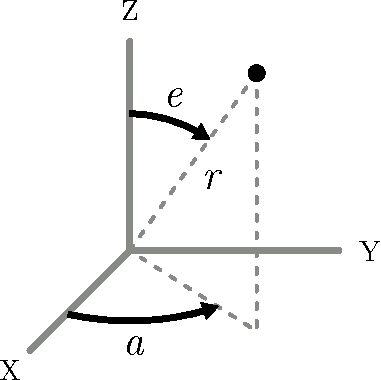
\includegraphics[width=.4\linewidth]{figures/sph_convention}
  \caption{Spherical grid definition and a spherical voxel}
  \label{fig:grid_details}
\end{figure}

\begin{table}[h]
  \centering
  \setlength{\tabcolsep}{4pt} % Default value: 6pt
  \caption{Spherical coordinate conventions.}
  \begin{tabular}{@{}lcccc@{}}
    \toprule
    \thead{Dimension} &
    \thead{Physics \\ Convention} &
    \thead{Math \\ Convention} &
    \thead{Manuscript \\ Convention} &
    \thead{Manuscript \\ Range} \\
    \midrule
        Radial & $r$ & $r$ & $r$ & [3 Re, 25 Re] \\
        Elevational & $\theta$ & $\phi$ & $e$ & [0°, 180°] \\
        Azimuthal & $\phi$ & $\theta$ & $a$ & [-180°, 180°] \\
    \botrule
  \end{tabular}
  \label{tab:sph_convention}
\end{table}

The grid resolution necessary to avoid aliasing and sample errors is data-dependent and was selected by exhaustive search to keep introduced error small.

\subsection{Inverse Problem}

Under the conditions described in Section \ref{sec:measurement_constraints} (single scattering in an optically-thin exosphere) and ignoring noise, tomographic inversion can be formulated as the solution of the linear inverse problem

$$\bm{y} = F \bm{\rho}$$

with measurements $\bm{y}$, forward operator $F$, and density $\bm{\rho}$.

Direct inversion of the tomographic operator requires that the matrix $F$ be non-singular in order for an inverse $F^{-1}$ to exist.  However, tomography problems generally have fewer measurement constraints LOS than free variables (voxels), making them ill-posed (lacking existence, uniqueness or stability of solutions).


While inversion of $F$ is impossible, the problem of obtaining estimate $\hat{\bm{\rho}}$ is sometimes reformulated as a minimization of some objective function, such as the common least squares

\begin{equation*}
  \hat{\bm{\rho}} = R(\bm{y}) = \min_{\bm{\rho}} || \bm{y} - F \bm{\rho} ||_2^2
\end{equation*}
\label{eqn:cost_function}

A generalized inverse such as the Moore-Penrose pseudoinverse, can be constructed from $F$ which selects the solution $\bm{\rho}$ with the smallest norm or which best fits the measurements.  Another approach is to assume that $\bm{\rho}$ has some low degree-of-freedom representation on a subspace (linear) or manifold (non-linear) within the space of all solutions.  Such a mapping $M$ is referred to as a model in this manuscript and is represented as

  $$\bm{\rho} = M(\bm{c})$$

where $\bm{c}$ are the low degree-of-freedom coefficients.  If the model is sufficiently low-dimensional and linear, then uniqueness is guaranteed if a solution exists.

However, this solution may still be ill-conditioned, or unstable in the presence of noise.  In these cases, $F$ is usually rank-deficient or has small singular values meaning that small perturbations in the measurements $\bm{y}$ are amplified greatly in the inversion process.
    This is especially true of computational imaging problems like tomography, where smoothing effects of integration dampen the high frequency information about $\bm{\rho}$ available in the measurements.


A common technique for addressing instability is to add additional terms to Equation \ref{eqn:cost_function} which encode prior knowledge about the distribution of $\bm{\rho}$ which may not be captured by the model.  This is known as regularization and can be used to combat ill-posedness.
  An alternative approach is to view inverse problems as a probabilistic inference problem which uses Bayes theorem to model uncertainty in reconstruction $\bm{\rho}$ given measurements $\bm{y}$.

The issues of solution existence, uniqueness and sensitivity in inverse problems were formally described by Hadamard in the early 20th century and used to define ill-posed and ill-conditioned inverse problems \cite{hadamard} \cite{illposed}.

    The notation introduced in this section is summarized in Table \ref{tab:symbols} and will be used throughout the manuscript.

  These principles of solution models and regularization have been used historically to guide retrieval algorithms and will be utilized
  by Carruthers for retrieval of exospheric density, described in
  (FIXME static-retrieval section reference).


The next section will cover the implementation of forward operator $F$, a critical component of tomographic retrieval which must be implemented efficiently when solving the objective function in an iterative manner.

\begin{table*}[!t]
  \centering
  %% \setlength{\tabcolsep}{4pt} % Default value: 6pt
  \setlength{\extrarowheight}{6pt}
  \caption{Symbols}
  \begin{tabular}{l c m{15em} m{12em}}
    \toprule
    \thead{Symbol} & \thead{Meaning} & \thead{Description} & \thead{Shape} \\
    \midrule
      $F$ & Forward operator & Mapping from 3D H density \newline to measurement stack & $F: \bb{R}^3 \rightarrow \bb{R}^3$ (static) \newline $F: \bb{R}^4 \rightarrow \bb{R}^3$ (dynamic) \\
    $M$ & Model & Mapping from model \newline parameters to 3D H density & $M: \bb{R}^* \rightarrow \bb{R}^3$ (static) \newline $M: \bb{R}^* \rightarrow \bb{R}^4$ (dynamic) \\

    $\bm{c}$ & Model params./coeffs. & Free model variables \& usually low-dimensional. & $\bm{c} \in \bb{R}^*$ \* model dependent \\

    $\bm{\rho}$ & H density & Spatial distribution of \newline exospheric hydrogen & $\bm{\rho} \in \bb{R}^3$ (static) \newline $\bm{\rho} \in \bb{R}^4$ (dynamic) \\
    $\bm{y}$ & Measurements & Column densities measured by instrument & $\bm{y} \in \bb{R}^3$ \\
    $R$ & Retrieval algorithm & Mapping from measurement stack to 3D H density & $R: \bb{R}^3 \rightarrow \bb{R}^3$ (static) \newline $R: \bb{R}^3\rightarrow\bb{R}^4$ (dynamic) \\
    $\hat{\circ}$ & Retrieved & Indicates estimated quantity\ (rather than ground truth) & \\
    \botrule
  \end{tabular}
  \label{tab:symbols}
\end{table*}

% ========================= RECONSTRUCTION MODEL ===================

\section{Spherical Harmonic Spline Representation}
\label{sec:shsr}

Zoennchen et al. \cite{zoennchen_new} present a retrieval method (derived from earlier work \cite{zoennchen2011}, \cite{zoennchen2013}, \cite{zoennchen_old}) featuring a partially separable parametric model based on a spherical harmonic representation (SHR).  Partially separable means the model can be expressed as a product of lower-dimensional functions which can decrease computational requirements.
Spherical harmonics are a family of complex, two-dimensional, continuous, orthonormal functions defined over a spherical domain.  These functions are commonly used in planetary atmospheric sciences \cite{hodges}, atomic physics (electron orbitals), computer graphics and more.  They serve as an analog to the Fourier basis in a spherical domain and approximate smoothly-varying spherical functions by linear combination of the basis.

%% // FIXME: ital degree order

Spherical harmonics are typically denoted $Y_(l m)(e, a)$ where $l$ and $m$ are known as the function degree and order.  In planetary physics, the convention is to denote coefficients of this linear combination as $A_(l m)$ (when $m \geq 0$) and $B_{l m}$ (when $m < 0$).  Figure \ref{fig:sph_harm} gives a graphical overview of the real/imaginary parts of the first few degrees of spherical harmonic functions.

\begin{figure}[h]
  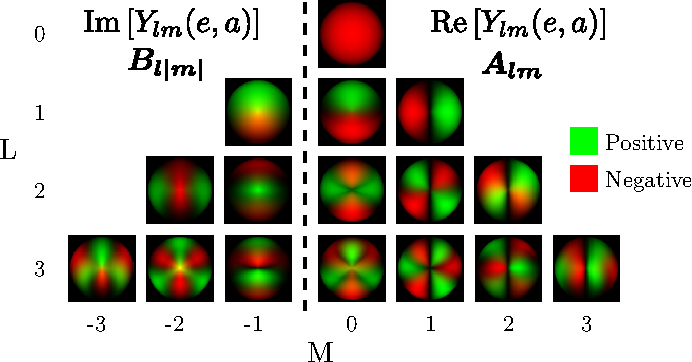
\includegraphics[width=1\linewidth]{figures/harm}
  \caption{First 3 degrees of spherical harmonic functions}
  \label{fig:sph_harm}
\end{figure}

The model density distribution assumed by Zoennchen et al. \cite{zoennchen_new} is given as

\begin{equation}
  n_H (r, e, a) = c r^{-k} d^{1/r} \text{SHR}(r, e, a)
  \label{eqn:radial_decay}
\end{equation}


Previous models are either incapable of representing spherical asymmetries, require a density prior (problematic for an understudied atmospheric regime), or lack the interpretability of a spherical harmonic basis.
This method replaces the relatively strong assumption of an inverse power law governing radial density variation with a more adaptable cubic spline model.
This formulation is less strict about the shape of radial density profiles but still enforces smoothness of spherical harmonic coefficients.

This section describes a new partially separable model which uses spherical harmonics as basis functions like the one used by Zoennchen et al.

The density model is written as

\begin{align}
  M(\bm{c}) &:= H S \bm{c} = \sum_{l=0}^L \sum_{m=-l}^l H_{l m}(e, a) S_{l m}(r) \\
  S_{l m}(r) &= \sum_{k=1}^K c_{l m k} B_{k 2}(r)
\end{align}

\begin{equation}
  H_{l m}(e, a) =
  \begin{cases}
    \text{Re}[Y_{l m}(e, a)] \text{ if } m \geq 0 \\
    \text{Im}[Y_{l m}(e, a)] \text{ if  } m < 0 \\
  \end{cases}
\end{equation}

  where $S_{l m}(r)$ is a cubic spline function composed of $K$ third order B-splines ${B_{1 2}, ...}$ that define spherical harmonic coefficients between $K$ radially log-spaced control point shells, illustrated in Figure \ref{fig:sph_harm_spline} with truncation order $L=3$.  This basis function formulation for $H_{l m}$ is equivalent to the one presented above but avoids notational awkwardness when $m \geq 0$ versus $m < 0$.


\begin{figure}[h]
  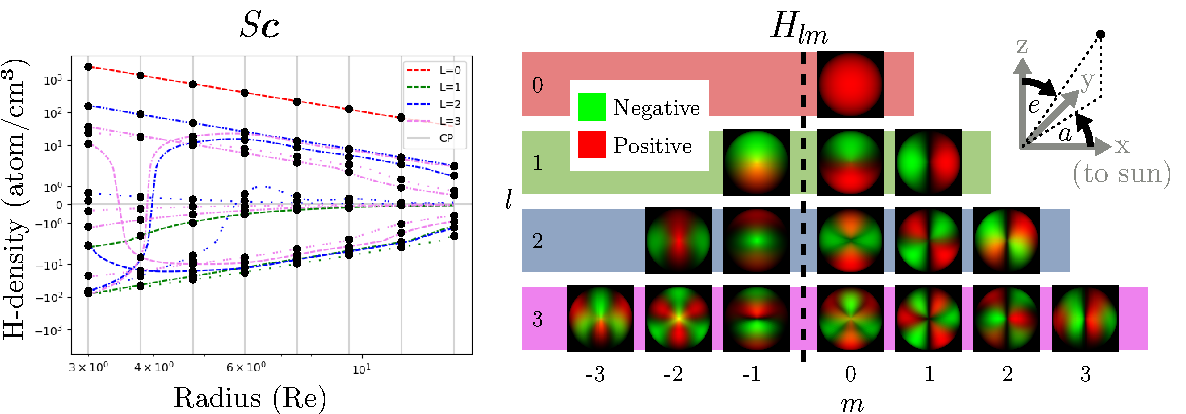
\includegraphics[trim={0 0 12cm 0},clip,width=1\linewidth]{figures/harm_spline}
  \caption{Smooth variation of coefficients in radial direction enforced by B-splines}
  \label{fig:sph_harm_spline}
\end{figure}

The spherical harmonic functions are aligned to the GSE coordinate system, with +Z as the primary axis of symmetry and the positive bulge of $H_(1 1)$ oriented towards the Sun in the +X direction.

The number and location of the $K$ control points used in the spline functions and the maximum spherical harmonic degree $L$ are selected at model initialization time.

(FIXME - remove this) static-justification justifies specific choices of $K$ and $L$ for the Carruthers mission.

The model inputs are $\bm{c} = \{c_{0 0 0}, ...\}$ and the minimization problem is

\begin{align}
    \hat{\bm{c}} =& \arg \min_{\bm{c}} ||\bm{y} - F(M(\bm{c}))||_1 \notag \\
    &+ \lambda_1 ||S(\bm{c})||_1 + \lambda_2 ||\text{clip}_{(-\infty, 0)}(M(\bm{c}))||_1
    \label{eqn:sphharmspline_min}
\end{align}

\begin{equation}
  \bm{\hat{\rho}} = M(\bm{\hat{c}})
\end{equation}

    Equation \ref{eqn:sphharmspline_min} uses an $L_1$ fidelity loss for robustness against outliers in measurements $\bm{y}$, an $L_1$ regularization (LASSO) on spline-interpolated coefficients for model interpretability, and an $L_1$ penalization term on negative densities to enforce model correctness.
    Note that a choice of $L=0$ enforces spherical symmetry, which can be useful for single snapshot retrievals.

    Because of the generalizability of spline density profiles and interpetability of spherical harmonics by the atmosphere science community, this is the primary method that will be used by the Carruthers mission for retrieving exospheric density during exospheric quiet conditions.

%% ===================== UNCERTAINTY QUANTIFICATION ====================


\section{Uncertainty Quantification}

Factors such as solar g factor, instrument radiation levels and detector health can influence measurement SNR and therefore the quality of the H density reconstructions.  Additionally, the posedness of the inverse problem introduced in Section \ref{sec:inverse_problem} is vantage-dependent resulting in increased reconstruction error for exospheric regions with poor LOS coverage from the given vantage.

To improve the scientific value of retrievals and aid in their interpretability, the data products will include an uncertainty map in the same shape as the H density data products which describes an estimated variance of the H density in each voxel.
This uncertainty map will be computed by Monte Carlo simulation from an ensemble of synthetic measurements $\{\bm{y'}_1, \bm{y'}_2, ...\}$.  These synthetic measurements will be generated in a bootstrapping process \cite{bootstrap} by resampling a real measurement $\bm{y}$ and knowledge of the instrument model.
This uncertainty map is too expensive to generate for every retrieval, so the Monte Carlo simulation will run at a reduced cadence and should remain valid for short timescales under identical storm conditions.

%% ===================== RESULTS AND DISCUSSION ====================

\section{Results and Discussion}

The retrieval algorithm implicitly encodes assumptions about hydrogen density distribution (smoothness, spherical harmonic structures, etc.), and verification that these assumptions hold requires testing against plausible ground truth densities.  This section overviews some of the ground truth datasets that are available for validation, their origins, spatiotemporal coverage, and model assumptions.

    FIXME - delete - Zoennchen \& TWINS

    Using the parametric model described in \cite{zoennchen_new}, Zoennchen et. al fit several density distributions to Lyman-$\alpha$ radiance measurements observed by TWINS from specific days in both solar minimum and maximum conditions during geomagnetic quiet conditions near Summer solstice.
    Notably, this dataset (referred to as the TWINS SPH dataset) was generated from the spherical harmonic model described in Section \ref{sec:shsr} with order L=3 and stronger assumptions about radial decay of hydrogen distribution.

  FIXME - delete - Vidal-Madjar and Bertaux

  Another validation dataset which will be referred to as the VMB (Vidal-Madjar \& Bertaux) model \cite{vmb} is a physics-based simulation of the exosphere.  It takes as input 2D temperature and H density distributions at the exobase (derived from NRLMSIS 2.0 \cite{msis}) and propagates this H density upwards and laterally.  By choosing different dates of the MSIS inputs, the model supports generating both geomagnetically quiet and storm-condition densities.  This simulation utilizes Louisville's equation to propagate constraints from the exobase, ignoring physical processes which are known to influence exospheric hydrogen distribution at large radial distances, such as solar radiation pressure and charge-exchange.

  Table \ref{tab:datasets} gives an overview of these datasets.

\begin{table*}[h]
  \centering
  %% \setlength{\tabcolsep}{4pt} % Default value: 6pt
  \caption{Synthetic ground-truth datasets}%
  \begin{tabular}{@{}lcccc@{}}
    \toprule
    %% Camera & FOV (degrees) & Resolution (pixels) & Angular Res. (degrees) & Spatial Res. (Re, proj.) & FOV Radius (min-max Re) \\
    \thead{Dataset} &
    \thead{Dynamic/Static} &
    \thead{Derived from} &
    \thead{Storm Condition} &
    \thead{Coverage} \\
    \midrule
    TWINS SPH \cite{zoennchen_new} & Static & Data \newline (TWINS) & Quiet & 3-25 Re \\
    VMB \cite{vmb} & Dynamic & Simulation & Quiet/Storm & 3-15 Re \newline 1 year (daily) \\
    \botrule
  \end{tabular}
  \label{tab:datasets}
\end{table*}


  FIXME: delete - Retrieval Performance retrieval-validation

  The Spherical Harmonic Spline method introduced in \ref{sec:shsr} will be used by the Carruthers mission for retrieval of the exospheric H density distribution during both geomagnetically active and quiet conditions.  During geomagnetically quiet conditions, the exosphere evolves slowly enough that the H density distribution may be considered static over a 2 week window of evolving vantages.  This window provides sufficient measurement diversity to capture small-scale structures within the density distribution, so Carruthers will use a spherical harmonic truncation order of L=3 during these periods.

  Figures \ref{fig:recon2w_twins} and \ref{fig:recon2w_vmb} give accuracy error for a single static density retrieval over a 2 week observation window with evolving vantage on the TWINS SPH and VMB datasets.  The "true" coefficients are a direct least-squares fit of the Spherical Harmonic Spline model to the dataset 3D densities without forward model or noise.
  Notably, the retrieval error is the smallest in the transverse (YZ) plane which is especially noticeable in the VMB retrieval.  This plane is oriented roughly perpendicular to measured LOS, which intuitively should give good conditioning, and thus high-quality retrievals, to voxels in this region.  Vertical gray bars indicate the location of spline control points.

    Additionally, errors are larger in the low-altitude region near the midnight (-X) side of Earth, where no LOS intersect due to occlusion by the Earth and optically-thick exosphere.  Voxels in this region are constrained only by spatial smoothing in the reconstruction model.


\begin{figure}[ht]
  \centering
  \begin{subfigure}[t]{1\linewidth}
    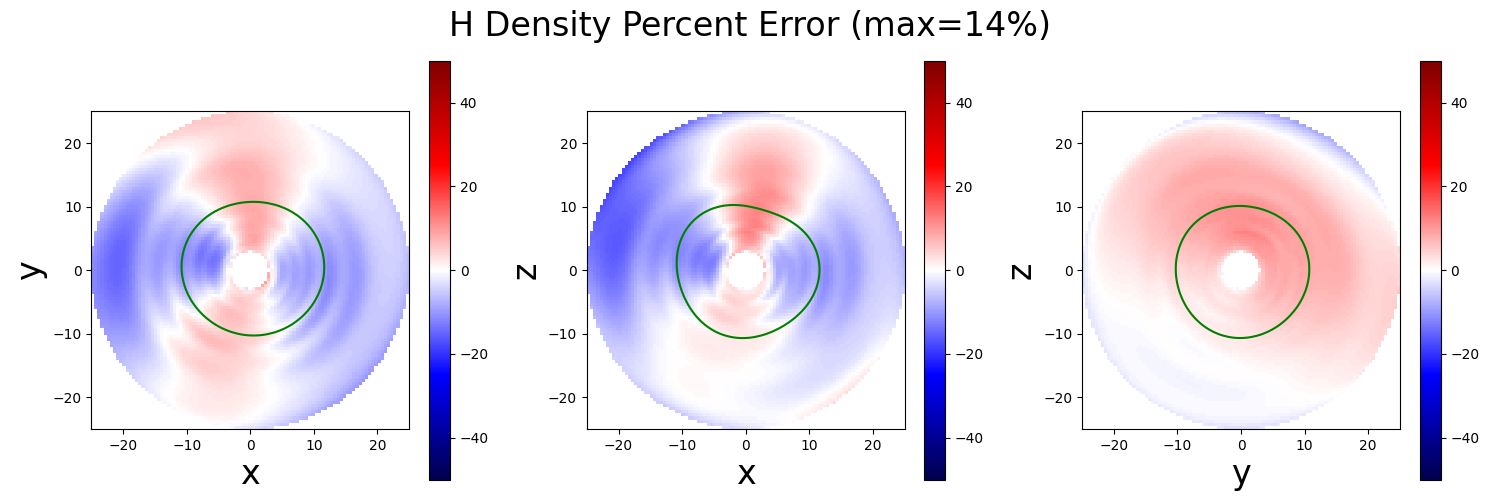
\includegraphics[height=1.2in]{figures/recon2w_twins_err}
    \caption{Reconstruction Error}
  \end{subfigure}%
  \newline
  \begin{subfigure}[t]{0.45\linewidth}
    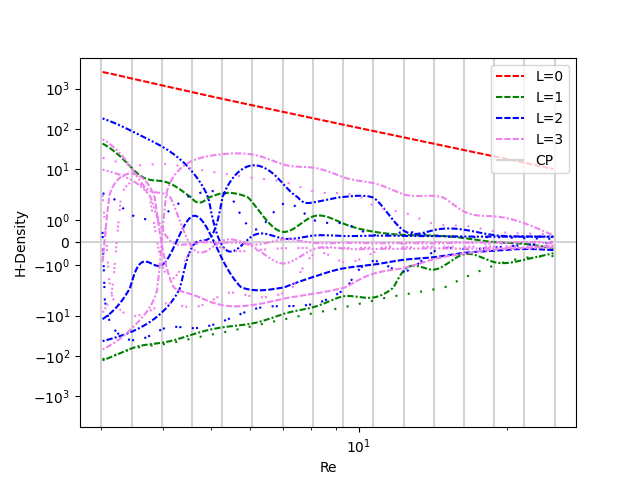
\includegraphics[height=1.3in]{figures/recon2w_twins_coeffs}
    \caption{Recon. coefficients}
  \end{subfigure}
  \begin{subfigure}[t]{0.45\linewidth}
    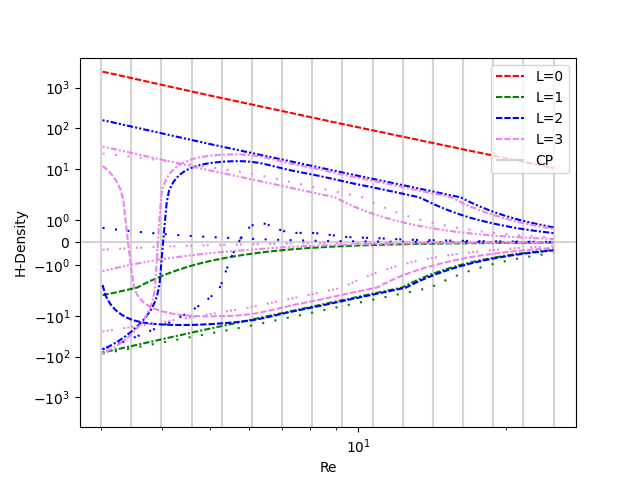
\includegraphics[height=1.3in]{figures/recon2w_twins_coeffs_truth}
    \caption{True coefficients}
  \end{subfigure}
  \caption{Two week TWINS SPH reconstruction results}
  \label{fig:recon2w_twins}
\end{figure}

\begin{figure}[ht]
  \centering
  \begin{subfigure}[t]{1\linewidth}
    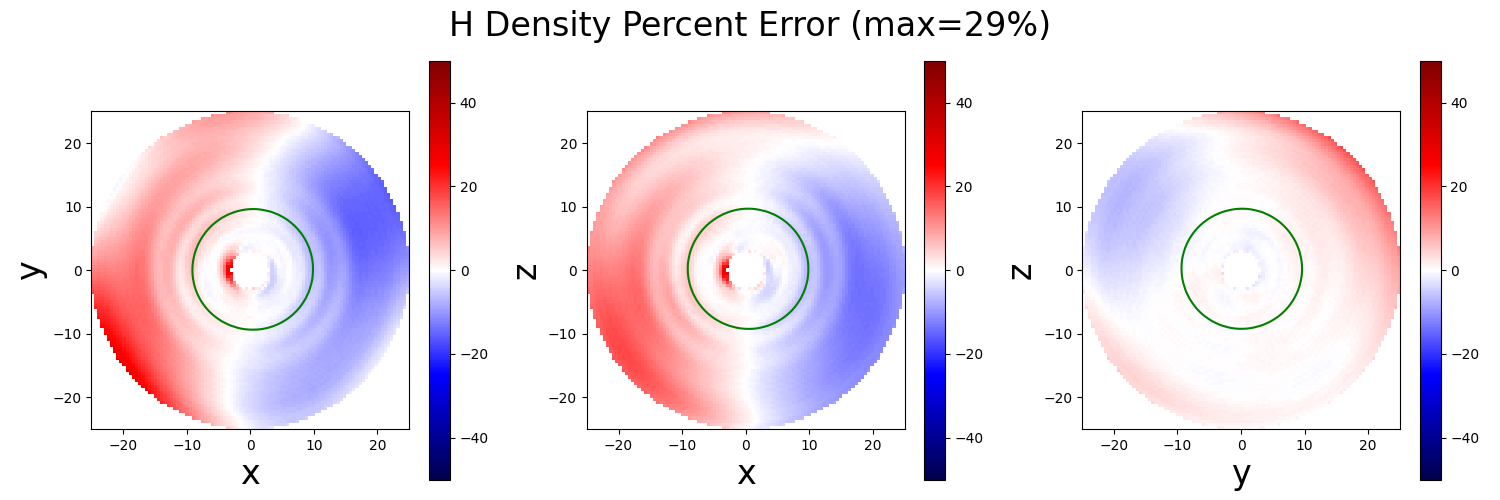
\includegraphics[height=1.2in]{figures/recon2w_vmb_err}
    \caption{Reconstruction Error}
  \end{subfigure}%
  \newline
  \begin{subfigure}[t]{0.45\linewidth}
    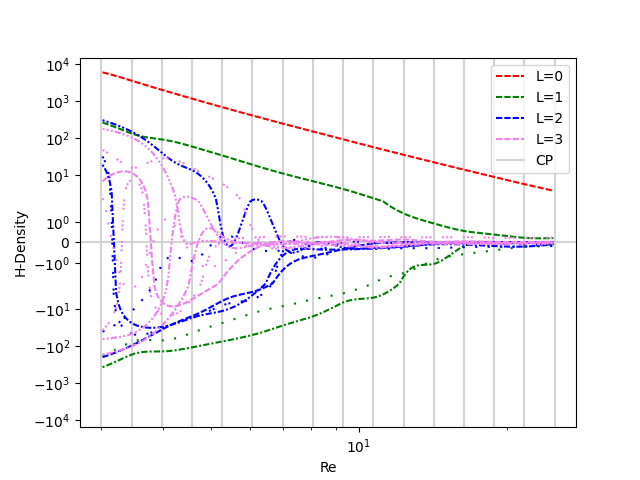
\includegraphics[height=1.3in]{figures/recon2w_vmb_coeffs}
    \caption{Recon. coefficients}
  \end{subfigure}
  \begin{subfigure}[t]{0.45\linewidth}
    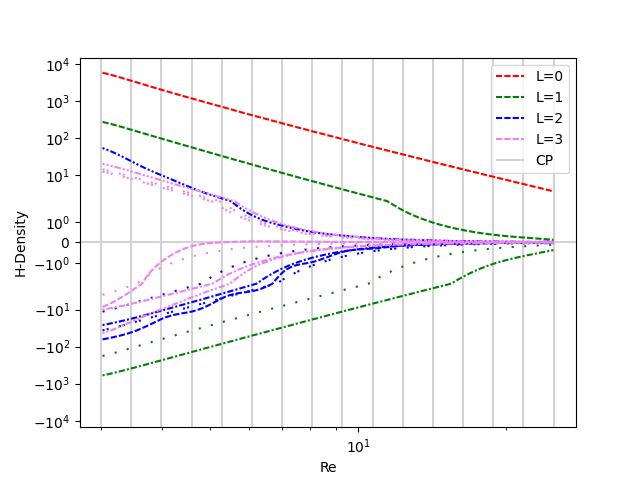
\includegraphics[height=1.3in]{figures/recon2w_vmb_coeffs_truth}
    \caption{True coefficients}
  \end{subfigure}
  \caption{Two week VMB reconstruction results}
  \label{fig:recon2w_vmb}
\end{figure}


  This test was repeated for 50 trials to establish that accuracy requirements are met at the necessary confidence level, shown in \ref{fig:recon2w_twins_montecarlo}.
    The complete model parameters (e.g. control points, spherical harmonic order, etc.) and experimental settings (e.g. grid and view geometry resolution) used for reconstructing both of these cases is given in \ref{tab:quiet_recon_params}.

\begin{figure}[h]
  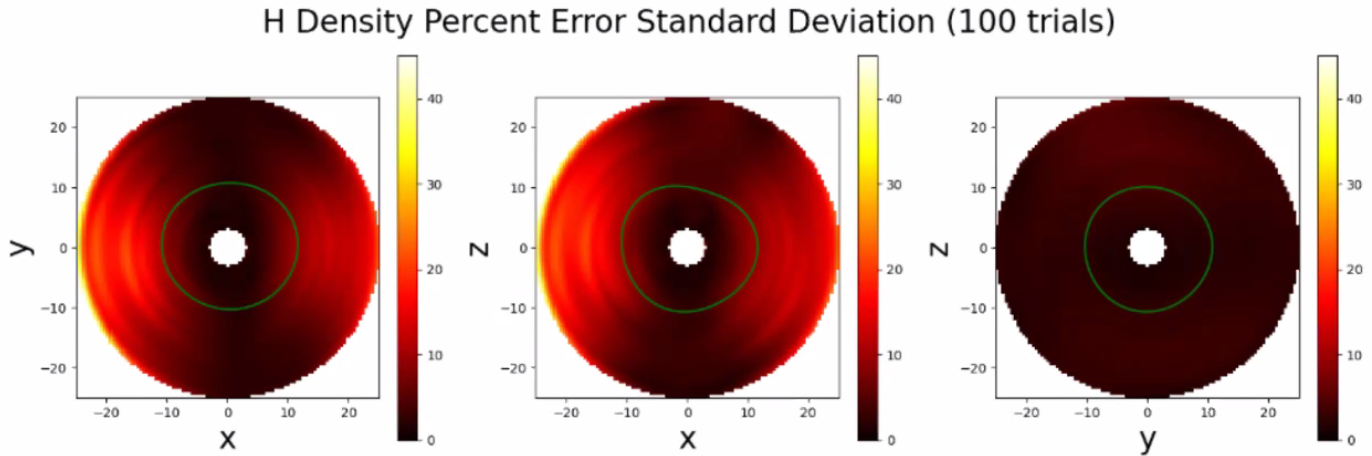
\includegraphics[width=1\linewidth]{figures/recon2w_twins_montecarlo}
  \caption{Two week reconstruction error standard deviation (percent).  50 reconstruction trials with separate noisy measurement realizations.}
  %% \footnotetext{Earth/Moon image courtesy of https://de.wikipedia.org/wiki/Benutzer:Master_Uegly}
  \label{fig:recon2w_twins_montecarlo}
\end{figure}

\begin{table*}[h!]
  \centering
  %% \setlength{\tabcolsep}{4pt} % Default value: 6pt
  \caption{Reconstruction parameters}%
  \begin{tabular}{@{}cccccc@{}}
    \toprule
    %% Camera & FOV (degrees) & Resolution (pixels) & Angular Res. (degrees) & Spatial Res. (Re, proj.) & FOV Radius (min-max Re) \\
    \thead{Retrieval Parameter} &
    \thead{Value} \\
    \midrule
    Simulation Grid & (500, 45, 60) \\
    Reconstruction Grid & (200, 45, 60) \\
    View Geometry & (100, 50) \\
    Observation window & 14 days \\
    Harmonic Truncation Order (L) & 3 \\
    Harmonic Spline C. Points & 1 \\
    \botrule
  \end{tabular}
  \label{tab:quiet_recon_params}
\end{table*}

  During geomagnetic storms, the above static assumption no longer holds and the exosphere evolves significantly over a period of hours.  In these periods, Carruthers will use an observation window of 6 hours and limit truncation order to L=0 (spherically symmetric) to reflect the fact that poor measurement diversity of this short window cannot capture significant non-radial spatial variation.  Reconstruction results for this test are shown in \ref{fig:recon6h_twins} and \ref{fig:recon6h_vmb}.

  These results show that despite some non-spherical variation the TWINS SPH and VMB datasets are sufficiently spherically symmetric to be reconstructed with reasonable levels of error.  Notably, the reconstructed and ground truth L=0 coefficients are nearly a perfect match, which matches the expectation of a spherical symmetric retrieval model having good conditioning from nearly any vantage.

\begin{figure}[h]
  \centering
  \begin{subfigure}[t]{1\linewidth}
    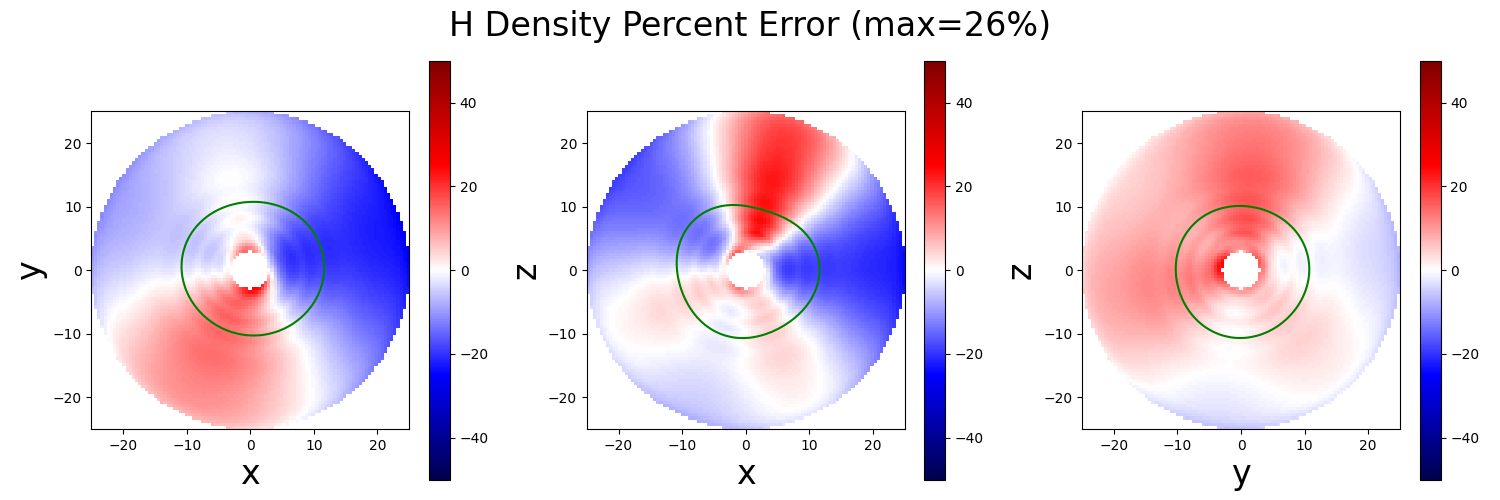
\includegraphics[height=1.2in]{figures/recon6h_twins_err}
    \caption{Reconstruction Error}
  \end{subfigure}%
  \newline
  \begin{subfigure}[t]{0.45\linewidth}
    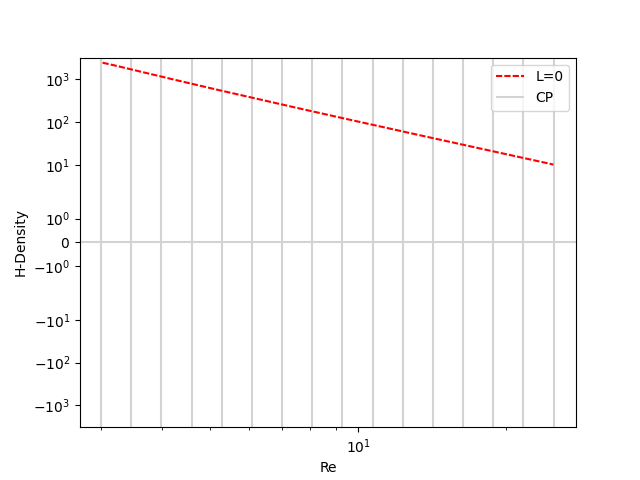
\includegraphics[height=1.3in]{figures/recon6h_twins_coeffs}
    \caption{Recon. coefficients}
  \end{subfigure}
  \begin{subfigure}[t]{0.45\linewidth}
    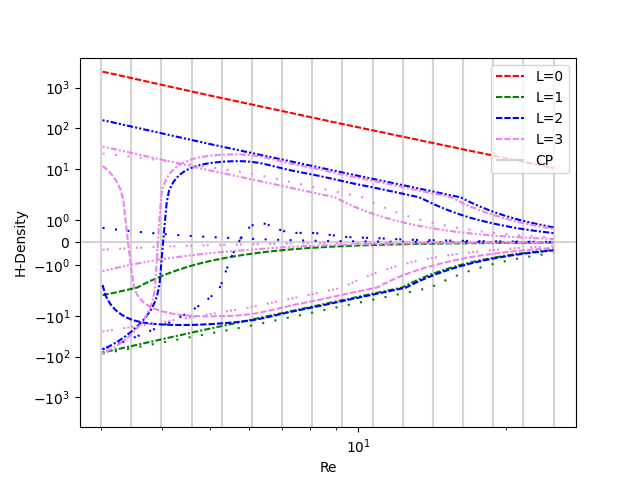
\includegraphics[height=1.3in]{figures/recon6h_twins_coeffs_truth}
    \caption{True coefficients}
  \end{subfigure}
  \caption{Six hour TWINS SPH reconstruction results}
  \label{fig:recon6h_twins}
\end{figure}

\begin{figure}[h]
  \centering
  \begin{subfigure}[t]{1\linewidth}
    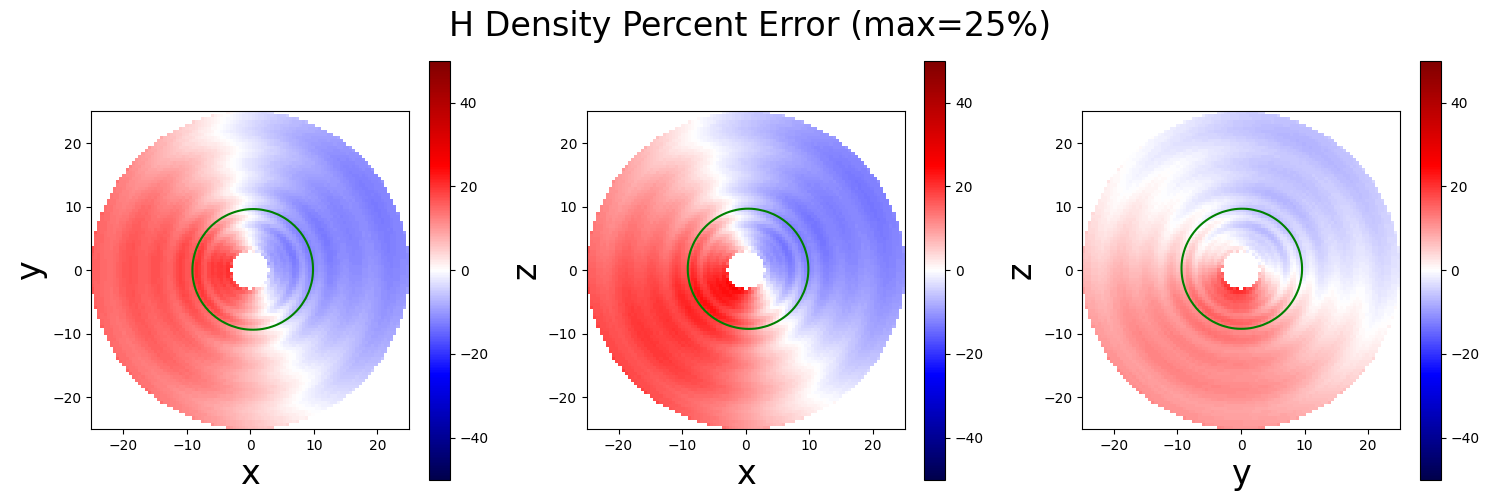
\includegraphics[height=1.2in]{figures/recon6h_vmb_err}
    \caption{Reconstruction Error}
  \end{subfigure}%
  \newline
  \begin{subfigure}[t]{0.45\linewidth}
    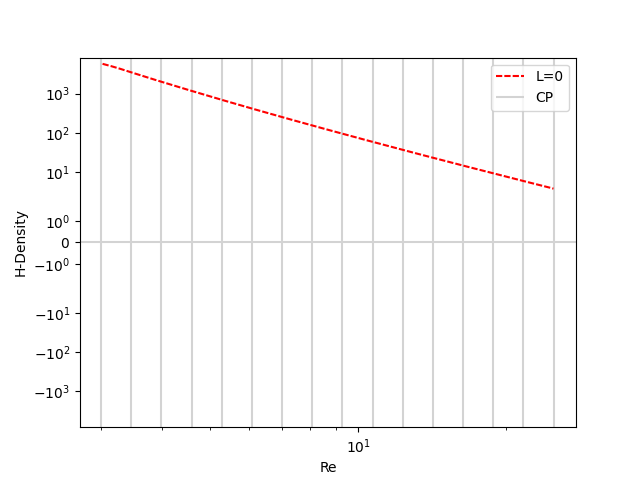
\includegraphics[height=1.3in]{figures/recon6h_vmb_coeffs}
    \caption{Recon. coefficients}
  \end{subfigure}
  \begin{subfigure}[t]{0.45\linewidth}
    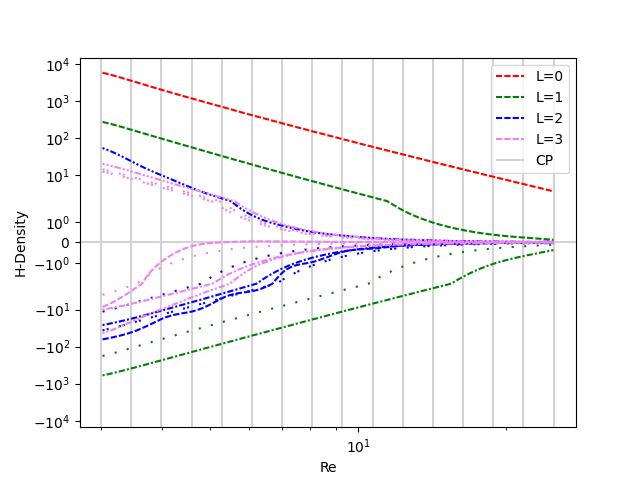
\includegraphics[height=1.3in]{figures/recon6h_vmb_coeffs_truth}
    \caption{True coefficients}
  \end{subfigure}
  \caption{Six hour VMB SPH reconstruction results}
  \label{fig:recon6h_vmb}
\end{figure}

  This section showed spherical harmonic model reconstruction results for both a large observation window suitable to geomagnetic quiet conditions, and a simpler spherically symmetric retrieval with a short window for storm conditions.  The reconstructions meet mission requirements [(FIXME) given in XXXXX] and were demonstrated to be stable across many reconstruction trials with different noisy measurement realizations.

%% ===================== CONCLUSION ====================

\section{Conclusion}

aaa \ref{tab:data_products}

\begin{table*}[h]
  \centering
  %% \setlength{\tabcolsep}{4pt} % Default value: 6pt
  \caption{Data products summary.  Altitude coverage is 3-25 Re.}%
  \begin{tabular}{@{}lcc@{}}
    \toprule
    %% Camera & FOV (degrees) & Resolution (pixels) & Angular Res. (degrees) & Spatial Res. (Re, proj.) & FOV Radius (min-max Re) \\
    \thead{Data Product} &
    \thead{Reporting Cadence \\ (minutes)} &
    \thead{Resolution \\ (voxels - rad., elev., azi.)} \\
    \midrule
    1D H Total & 30 & (200, 1, 1) \\
    1D Uncertainty & TBD & (200, 1, 1) \\
    3D H Total & 30 & (200, 45, 60) \\
    3D Uncertainty & TBD & (200, 45, 60) \\
    \botrule
  \end{tabular}
  \label{tab:data_products}
\end{table*}

\begin{appendices}

\section{Section title of first appendix}\label{secA1}

An appendix contains supplementary information that is not an essential part of the text itself but which may be helpful in providing a more comprehensive understanding of the research problem or it is information that is too cumbersome to be included in the body of the paper.

\end{appendices}

\bibliography{bibliography}

\end{document}